%iffalse
\let\negmedspace\undefined
\let\negthickspace\undefined
\documentclass[journal,12pt,onecolumn]{IEEEtran}
\usepackage{cite}
\usepackage{amsmath,amssymb,amsfonts,amsthm}
\usepackage{algorithmic}
\usepackage{graphicx}
\usepackage{textcomp}
\usepackage{mathrsfs}
\usepackage{xcolor}
\usepackage{txfonts}
\usepackage{listings}
\usepackage{enumitem}
\usepackage{mathtools}
\usepackage{gensymb}
\usepackage{comment}
\usepackage[breaklinks=true]{hyperref}
\usepackage{tkz-euclide} 
\usepackage{listings}
\usepackage{gvv}
\def\inputGnumericTable{}                                 
\usepackage[utf8]{inputenc}                              
\usepackage{color}                                         
\usepackage{array}                                        
\usepackage{longtable}                                     
\usepackage{calc}                                          
\usepackage{multirow}                                      
\usepackage{hhline}                                        
\usepackage{ifthen}                                        
\usepackage{lscape}
\newtheorem{theorem}{Theorem}[section]
\newtheorem{problem}{Problem}
\newtheorem{proposition}{Proposition}[section]
\newtheorem{lemma}{Lemma}[section]
\newtheorem{corollary}[theorem]{Corollary}
\newtheorem{example}{Example}[section]
\newtheorem{definition}[problem]{Definition}
\newcommand{\BEQA}{\begin{eqnarray}}
\newcommand{\EEQA}{\end{eqnarray}}
\newcommand{\define}{\stackrel{\triangle}{=}}
\theoremstyle{remark}
\newtheorem{rem}{Remark}
\graphicspath{ {./Figures/} }
\usepackage{float} % For the [H] float option
\usepackage{textcomp}
\usepackage{multicol}

\begin{document}
\begin{enumerate}[start=1, label=Q.\arabic*]

\item Rajiv Gandhi Khel Ratna Award was conferred \underline{\hspace{1cm}} Mary Kom, a six-time world champion in boxing, recently in a ceremony \underline{\hspace{1cm}} the Rashtrapati Bhawan \brak{\text{the President’s official residence}} in New Delhi.

\begin{enumerate}
\begin{multicols}{2}
\item with, at
\item on, in
\item on, at
\item to, at
\end{multicols}
\end{enumerate}

\hfill{\brak{\text{GATE MA 2020}}}

\item Despite a string of poor performances, the chances of K. L. Rahul’s selection in the team are \underline{\hspace{2cm}}.

\begin{enumerate}
\item slim
\item bright
\item obvious
\item uncertain
\end{enumerate}

\hfill{\brak{\text{GATE MA 2020}}}

\item Select the word that fits the analogy:  
Cover $:$ Uncover $:$$:$ Associate $:$ \underline{\hspace{2cm}}

\begin{enumerate}
\begin{multicols}{2}
\item Unassociate
\item Inassociate
\item Misassociate
\item Dissociate
\end{multicols}
\end{enumerate}

\hfill{\brak{\text{GATE MA 2020}}}

\item Hit by floods, the kharif \brak{\text{summer sown}} crops in various parts of the country have been affected. Officials believe that the loss in production of the kharif crops can be recovered in the output of the rabi \brak{\text{winter sown}} crops so that the country can achieve its food-grain production target of $291$ million tons in the crop year $2019$–$20$ \brak{\text{July–June}}. They are hopeful that good rains in July–August will help the soil retain moisture for a longer period, helping winter sown crops such as wheat and pulses during the November–February period.  

Which of the following statements can be inferred from the given passage?

\begin{enumerate}
\item Officials declared that the food-grain production target will be met due to good rains.
\item Officials want the food-grain production target to be met by the November–February period.
\item Officials feel that the food-grain production target cannot be met due to floods.
\item Officials hope that the food-grain production target will be met due to a good rabi produce.
\end{enumerate}

\hfill{\brak{\text{GATE MA 2020}}}

\item The difference between the sum of the first $2n$ natural numbers and the sum of the first $n$ odd natural numbers is \underline{\hspace{2cm}}.

\begin{enumerate}
\begin{multicols}{2}
\item $n^2 - n$
\item $n^2 + n$
\item $2n^2 - n$
\item $2n^2 + n$
\end{multicols}
\end{enumerate}

\hfill{\brak{\text{GATE MA 2020}}}

\item Repo rate is the rate at which Reserve Bank of India \brak{\text{RBI}} lends commercial banks, and reverse repo rate is the rate at which RBI borrows money from commercial banks.  

Which of the following statements can be inferred from the above passage?

\begin{enumerate}
\item Decrease in repo rate will increase cost of borrowing and decrease lending by commercial banks.  
\item Increase in repo rate will decrease cost of borrowing and increase lending by commercial banks.  
\item Increase in repo rate will increase cost of borrowing and decrease lending by commercial banks.  
\item Decrease in repo rate will decrease cost of borrowing and increase lending by commercial banks.  
\end{enumerate}

\hfill{\brak{\text{GATE MA 2020}}}

\item $P, Q, R, S, T, U, V$ and $W$ are seated around a circular table.  
I. $S$ is seated second place to the right of $R$.  
II. $V$ is seated at the third place to the left of $R$.  
III. $Q$ is a neighbour of $V$.  
IV. $R$ is a neighbour of $U$.  

Which of the following must be true?

\begin{enumerate}
\item $Q$ is a neighbour of $R$.  
\item $U$ is a neighbour of $S$.  
\item $P$ is not a neighbour of $R$.  
\item $P$ is the left neighbour of $R$.  
\end{enumerate}

\hfill{\brak{\text{GATE MA 2020}}}

\item The distance between Delhi and Agra is $233 \, \text{km}$. A car $P$ started travelling from Delhi to Agra and another car $Q$ started from Agra to Delhi along the same road $1 \, \text{hour}$ after the car $P$ started. The two cars crossed each other $75 \, \text{minutes}$ after the car $Q$ started. Both cars were travelling at constant speed. The speed of car $P$ was $10 \, \text{km/h}$ more than the speed of car $Q$. How many kilometers the car $Q$ had travelled when the cars crossed each other?

\begin{enumerate}
\begin{multicols}{2}
\item $66.2$  
\item $75.2$  
\item $85.8$  
\item $116.2$  
\end{multicols}
\end{enumerate}

\hfill{\brak{\text{GATE MA 2020}}}

\item For a matrix $M = \brak{m_{ij}}, i,j = 1,2,3,4$, the diagonal elements are all zero and $m_{ij} = -m_{ji}$. The minimum number of elements required to fully specify the matrix is \underline{\hspace{2cm}}.

\begin{enumerate}
\begin{multicols}{2}
\item $0$  
\item $6$  
\item $12$  
\item $16$  
\end{multicols}
\end{enumerate}

\hfill{\brak{\text{GATE MA 2020}}}

\item The profit shares of two companies $P$ and $Q$ are shown in the figure. If the two companies have invested a fixed equal amount every year, then the ratio of the total revenue of company $P$ to total revenue of company $Q$, during $2013$–$2018$, is \underline{\hspace{2cm}}.

\begin{figure}[H]
\centering
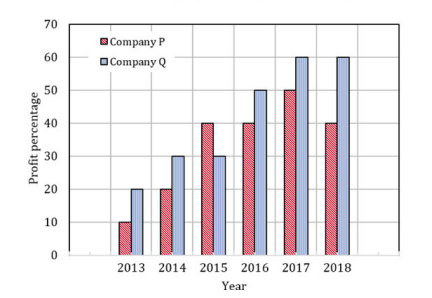
\includegraphics[width=0.7\columnwidth]{Figures/qs10.png}
\caption{}
\end{figure}

\begin{enumerate}
\begin{multicols}{2}
\item $15 : 17$  
\item $17 : 15$  
\item $17 : 13$  
\item $17 : 11$  
\end{multicols}
\end{enumerate}

\hfill{\brak{\text{GATE MA 2020}}}
\item Suppose that $d_1$, $d_2$ and $d_3$ are topologies on $X$ induced by metrics $d_1$, $d_2$ and $d_3$, respectively, such that $S_{d_1} \subseteq S_{d_2} \subseteq S_{d_3}$. Then which of the following statements is TRUE?

\begin{enumerate}
\item If a sequence converges in $\brak{X,d_2}$ then it converges in $\brak{X,d_1}$  
\item If a sequence converges in $\brak{X,d_3}$ then it converges in $\brak{X,d_2}$  
\item Every open ball in $\brak{X,d_1}$ is also an open ball in $\brak{X,d_2}$  
\item The map $x \mapsto x$ from $\brak{X,d_1}$ to $\brak{X,d_3}$ is continuous  
\end{enumerate}

\hfill{\brak{\text{GATE MA 2020}}}

\item Let $D = \brak{-1,1} \times \brak{-1,1}$. If the function $F : D \to \mathbb{R}$ is defined by  

\[
F\brak{x,y} = \begin{cases}
\dfrac{xy^2}{x^2+y^2}, & (x,y) \neq (0,0) \\
0, & (x,y) = (0,0)
\end{cases}
\]

then  
I. $F$ is continuous at $(0,0)$  
II. both the first order partial derivatives of $F$ exist at $(0,0)$  
III. $\iint_D |F(x,y)| \, dx\,dy$ is finite  
IV. $\iint_D F(x,y) \, dx\,dy$ is finite  

\begin{enumerate}
\item Only I and II are correct  
\item Only III and IV are correct  
\item I, II and III are correct  
\item All of I, II, III and IV are correct  
\end{enumerate}

\hfill{\brak{\text{GATE MA 2020}}}

\item The initial value problem  

\[
y' = y^2, \quad y(0) = b
\]

has  

\begin{enumerate}
\item a unique solution if $b=0$  
\item no solution if $b=1$  
\item infinitely many solutions if $b=2$  
\item a unique solution if $b=1$  
\end{enumerate}

\hfill{\brak{\text{GATE MA 2020}}}

\item Consider the following statements:  
I. $\log \brak{z}$ is harmonic on $\mathbb{C} \setminus \{0\}$  
II. $\log \brak{z}$ has a harmonic conjugate on $\mathbb{C} \setminus \{0\}$  

Then  

\begin{enumerate}
\item Both I and II are true  
\item I is true but II is false  
\item I is false but II is true  
\item Both I and II are false  
\end{enumerate}

\hfill{\brak{\text{GATE MA 2020}}}

\item Let $G$ and $H$ be defined by  

\[
G = \{ z = x+iy \in \mathbb{C} : x \cdot y = 0 \}, \quad  
H = \{ z = x+iy \in \mathbb{C} : x = 0, \, y \neq 0 \}
\]

Suppose $f : G \to \mathbb{C}$ and $g : H \to \mathbb{C}$ are analytic functions. Consider the following statements:  

I. $\int_{\gamma} f(z) \, dz$ is independent of path $\gamma$ in $G$ joining $-i$ and $i$  
II. $\int_{\gamma} g(z) \, dz$ is independent of path $\gamma$ in $H$ joining $-i$ and $i$  

Then  

\begin{enumerate}
\item Both I and II are true  
\item I is true but II is false  
\item I is false but II is true  
\item Both I and II are false  
\end{enumerate}

\hfill{\brak{\text{GATE MA 2020}}}
\item Let $f(n) = n^2, \, n \in \mathbb{Z}_{>0}$ and let, for $n \in \mathbb{N}$,

\[
R_n = \{ x+y\sqrt{2} : x,y \in \mathbb{Z}, \; |x| \leq n^2, \; |y| \leq n^2 \} \subseteq \mathbb{Q}(\sqrt{2}).
\]

If for a subset $S \subseteq \mathbb{R}$, $\overline{S}$ denotes the closure of $S$ in $\mathbb{R}$, then

\begin{enumerate}
\item $\overline{T\brak{\mathbb{Q}}} = T\brak{\mathbb{Q}}$  
\item $\overline{T\brak{R_n}} = T\brak{R_n}$  
\item $\overline{T\brak{\mathbb{Q}}} = \overline{T\brak{R_n}}$  
\item $\overline{T\brak{\mathbb{Q}}} = T\brak{R_n}$  
\end{enumerate}

\hfill{\brak{\text{GATE MA 2020}}}

\item Suppose that  

\[
U = \mathbb{R}^2 \setminus \{(x,y) \in \mathbb{R}^2 : x \cdot y = 0\}, \quad  
V = \mathbb{R}^2 \setminus \{(x,y) \in \mathbb{R}^2 : x \cdot y = 1\}.
\]

Then which one of the following statements is TRUE?  

\begin{enumerate}
\item Both $U$ and $V$ are bounded  
\item Both $U$ and $V$ are connected  
\item $U$ is connected but $V$ is disconnected  
\item $U$ is disconnected but $V$ is connected  
\end{enumerate}

\hfill{\brak{\text{GATE MA 2020}}}

\item Consider the two–dimensional dual problems of the linear programming problem  

\[
\text{(P1)} \quad \min z = x_1 + 2x_2, \quad \text{subject to } x_1 + x_2 \geq 1, \, x_1 \geq 0, \, x_2 \geq 0,
\]

\[
\text{(P2)} \quad \max w = y_1, \quad \text{subject to } y_1 \leq 1, \, y_1 + y_2 \leq 2, \, y_1, y_2 \geq 0.
\]

Then  

\begin{enumerate}
\item Both (P1) and (P2) are infeasible  
\item (P1) is infeasible and (P2) is feasible  
\item (P1) is feasible and bounded but (P2) is infeasible  
\item (P1) is feasible and unbounded but (P2) is feasible  
\end{enumerate}

\hfill{\brak{\text{GATE MA 2020}}}

\item If $f(x,y) = 5x + 6y - 6x^2 - 7xy - 2y^2 + 18y + x^3 + y^3$, where $(x,y) \in \mathbb{R}^2$, then  

\begin{enumerate}
\item $\brak{0,0}$ is a point of local maximum of $f$  
\item $\brak{0,0}$ is a saddle point of $f$  
\item $\brak{0,0}$ is a point of local minimum of $f$  
\item $\brak{0,0}$ is neither a local minimum nor a local maximum of $f$  
\end{enumerate}

\hfill{\brak{\text{GATE MA 2020}}}

\item Consider the iterative scheme  

\[
x_{n+1} = \dfrac{2}{3}x_n + \dfrac{1}{x_n^2}, \quad n \geq 1,
\]

with initial point $x_1 > 0$. Then the sequence $\{x_n\}$  

\begin{enumerate}
\item converges to $1$ if $x_1 > 0$  
\item converges to $2$ if $x_1 > 0$  
\item converges to $3$ if $x_1 > 0$  
\item does not converge for any $x_1 > 0$  
\end{enumerate}

\hfill{\brak{\text{GATE MA 2020}}}

\item Let $C[0,1]$ denote the space of all real–valued continuous functions on $\brak{0,1}$ equipped with the supremum norm $\|\cdot\|_\infty$. Let $T : C[0,1] \to C[0,1]$ be the linear operator defined by  

\[
T(f)(x) = \int_0^1 e^{xy} f(y) \, dy.
\]

Then  

\begin{enumerate}
\item $\|T\| = 1$  
\item $T^{-1}$ is not invertible  
\item $T$ is surjective  
\item $1 + \|T\| = 1 + \|T\|^2$  
\end{enumerate}

\hfill{\brak{\text{GATE MA 2020}}}

\item Suppose that $M$ is a $5 \times 5$ matrix with real entries and $p(x) = \det(xI-M)$. Then $p(x) = \det(M)$ if and only if  

\begin{enumerate}
\item Every eigenvalue of $M$ is real  
\item If $p(x) = 0$ then $p(x) + p(2) = 0 = p(2) + p(3)$  
\item $M^n$ is necessarily a polynomial in $M$ of degree $\leq 4$  
\item $M$ is invertible  
\end{enumerate}

\hfill{\brak{\text{GATE MA 2020}}}

\item Let $C[0,1]$ denote the space of all real–valued continuous functions on $\brak{0,1}$ equipped with the supremum norm $\|\cdot\|_\infty$. Let $f \in C[0,1]$ be such that  

\[
|f(x) - f(y)| \leq M |x-y|, \quad \forall \, x,y \in [0,1] \text{ and for some } M > 0.
\]

For $n \in \mathbb{N}$, let $S_n(f) = \{ f\brak{\tfrac{k}{n}} : k \in \mathbb{N}, k \leq n \}$. Then the closure of $S = \bigcup_{n \in \mathbb{N}} S_n(f)$  

\begin{enumerate}
\item is closed and bounded  
\item is bounded but not totally bounded  
\item is compact  
\item is closed but not bounded  
\end{enumerate}

\hfill{\brak{\text{GATE MA 2020}}}

\item Let $K : \mathbb{R} \times \brak{0,\infty} \to \mathbb{R}$ be a function such that the solution of the initial value problem  

\[
\frac{du(x)}{dx} = \int_0^\infty K(x-y) f(y) \, dy, \quad u(0) = f(x), \quad x \in \mathbb{R}, \; t \in (0,\infty),
\]

is given by  

\[
u(x,t) = \int_0^\infty K(x-y) f(y) \, dy
\]

for all bounded continuous functions $f$. Then the value of $\int_0^\infty K(x,y) \, dx$ is  

\begin{enumerate}
\item $0$  
\item $1$  
\item $2$  
\item $3$  
\end{enumerate}

\hfill{\brak{\text{GATE MA 2020}}}

\item The number of cyclic subgroups of the quaternion group  

\[
Q_8 = \{ a,b : a^4 = 1, \, a^2 = b^2, \, ba = a^{-1}b \}
\]

is \underline{\hspace{2cm}}.  

\begin{enumerate}
\begin{multicols}{2}
\item $5$  
\item $6$  
\item $7$  
\item $8$  
\end{multicols}
\end{enumerate}
\hfill{\brak{\text{GATE MA 2020}}}
\item The number of elements of order $3$ in the symmetric group $S_6$ is \underline{\hspace{2cm}}.

\begin{enumerate}
\begin{multicols}{2}
\item $20$
\item $40$
\item $60$
\item $80$
\end{multicols}
\end{enumerate}

\hfill{\brak{\text{GATE MA 2020}}}

\item Let $F$ be the field with $4096$ elements. The number of proper subfields of $F$ is \underline{\hspace{2cm}}.

\begin{enumerate}
\begin{multicols}{2}
\item $2$
\item $3$
\item $4$
\item $5$
\end{multicols}
\end{enumerate}

\hfill{\brak{\text{GATE MA 2020}}}

\item If $(x_1, x_2^*)$ is an optimal solution of the linear programming problem,

\[
\text{minimize } \; x_1 + 2x_2
\]

subject to  

\[
\begin{aligned}
4x_1 - x_2 &\geq 8 \\
2x_1 + x_2 &\geq 10 \\
-x_1 + x_2 &\leq 7 \\
x_1, x_2 &\geq 0
\end{aligned}
\]

and $(\lambda_1^*, \lambda_2^*, \lambda_3^*)$ is an optimal solution of its dual problem, then  
\[
\sum_{i=1}^2 x_i^{*2} + \sum_{j=1}^3 \lambda_j^{*2}
\]
is equal to \underline{\hspace{2cm}} (correct up to one decimal place).

\begin{enumerate}
\item $20.2$
\item $21.6$
\item $22.3$
\item $23.8$
\end{enumerate}

\hfill{\brak{\text{GATE MA 2020}}}

\item Let $a, b, c \in \mathbb{R}$ be such that the quadrature rule  

\[
\int_{-1}^1 f(x) \, dx \approx af(-1) + bf(0) + cf(1)
\]

is exact for all polynomials of degree less than or equal to $2$. Then $b$ is equal to \underline{\hspace{2cm}} (rounded off to two decimal places).

\begin{enumerate}
\begin{multicols}{2}
\item $1.33$
\item $1.67$
\item $2.00$
\item $2.33$
\end{multicols}
\end{enumerate}

\hfill{\brak{\text{GATE MA 2020}}}

\item Let $f(x) = x^4$ and let $p(x)$ be the interpolating polynomial of $f$ at nodes $1,2$ and $3$. Then $p(0)$ is equal to \underline{\hspace{2cm}}.

\begin{enumerate}
\begin{multicols}{2}
\item $-2$
\item $-4$
\item $-6$
\item $-8$
\end{multicols}
\end{enumerate}

\hfill{\brak{\text{GATE MA 2020}}}

\item For $n \geq 2$, define the sequence $\{x_n\}$ by  

\[
x_n = \frac{1}{2\pi} \int_0^{\pi/2} \tan^n t \, dt.
\]

Then the sequence $\{x_n\}$ converges to \underline{\hspace{2cm}} (correct up to two decimal places).

\begin{enumerate}
\begin{multicols}{2}
\item $0.50$
\item $0.75$
\item $1.00$
\item $1.25$
\end{multicols}
\end{enumerate}

\hfill{\brak{\text{GATE MA 2020}}}

\item Let 
\[
L^2[0,10] = \{ f : [0,10] \to \mathbb{R} : f \text{ is Lebesgue measurable and } \int_{0}^{10} f^2 dx < \infty \}
\] 
equipped with the norm 
\[
\abs{f} = \brak{\int_{0}^{10} f^2 dx}^{\tfrac{1}{2}}
\] 
and let $T$ be the linear functional on $L^2[0,10]$ given by 
\[
T(f) = \int_{0}^{2} f(x)dx - \int_{3}^{10} f(x)dx.
\]  

Then $\abs{T}$ is equal to \underline{\hspace{2cm}}

\hfill{\brak{\text{GATE MA 2020}}}


\item If $\{x_{13}, x_{22}, x_{23} = 10, x_{31}, x_{32}, x_{34}\}$ is the set of basic variables of a balanced transportation problem seeking to minimize cost of transportation from origins to destinations, where the cost matrix is,  

\begin{table}[H]
\centering
\begin{tabular}{|c|c|c|c|c|c|}
\hline
 & $D_1$ & $D_2$ & $D_3$ & $D_4$ & \text{Availability} \\ \hline
$O_1$ & $6$ & $2$ & $-1$ & $0$ & $10$ \\ \hline
$O_2$ & $4$ & $2$ & $2$ & $3$ & $\lambda + 5$ \\ \hline
$O_3$ & $3$ & $1$ & $2$ & $1$ & $3\lambda$ \\ \hline
\text{Demand} & $10$ & $\mu - 5$ & $\mu + 5$ & $15$ & \\ \hline
\end{tabular}
\caption*{}
\label{tab:transport}
\end{table}

and $\lambda, \mu \in \mathbb{R}$, then $x_{32}$ is equal to \underline{\hspace{2cm}}

\hfill{\brak{\text{GATE MA 2020}}}

\item Let $\mathbb{Z}_{225}$ be the ring of integers modulo $225$. If $x$ is the number of prime ideals and $y$ is the number of nontrivial units in $\mathbb{Z}_{225}$, then $x+y$ is equal to \underline{\hspace{2cm}}.

\hfill{\brak{\text{GATE MA 2020}}}

\item Let $u\brak{x,t}$ be the solution of
\begin{align*}
\frac{\partial^{2}u}{\partial t^{2}}-\frac{\partial^{2}u}{\partial x^{2}}&=0,\\
u\brak{x,0}&=f\brak{x},\\
\frac{\partial u}{\partial t}\brak{x,0}&=0,\quad x\in\mathbb{R},\ t>0,
\end{align*}
where $f$ is a twice continuously differentiable function. If $f\brak{-2}=4$, $f\brak{0}=0$, and $u\brak{2,2}=8$, then the value of $u\brak{1,3}$ is \underline{\hspace{2cm}}.

\hfill{\brak{\text{GATE MA 2020}}}

\item Let $\{e_n\}_{n=1}^{\infty}$ be an orthonormal basis for a separable Hilbert space $H$ with the inner product $\langle\,\cdot,\cdot\,\rangle$. Define
\[
f_n=e_n-\frac{1}{n+1}e_{n+1}\quad \text{for } n\in\mathbb{N}.
\]
Then
\begin{enumerate}
\item the closure of the span $\{f_n: n\in\mathbb{N}\}$ equals $H$
\item $f=0$ if $\langle f,f_n\rangle=\langle f,e_n\rangle$ for all $n\in\mathbb{N}$
\item $\{f_n\}_{n=1}^{\infty}$ is an orthogonal subset of $H$
\item there does not exist nonzero $f\in H$ such that $\langle f,e_2\rangle=\langle f,f_2\rangle$
\end{enumerate}

\hfill{\brak{\text{GATE MA 2020}}}

\item Suppose $V$ is a finite dimensional nonzero vector space over $\mathbb{C}$ and $T: V\to V$ is a linear transformation such that $\text{Range}\brak{T}=\text{Nullspace}\brak{T}$. Then which of the following statements is \text{FALSE}?
\begin{enumerate}
\item the dimension of $V$ is even
\item $0$ is the only eigenvalue of $T$
\item both $0$ and $1$ are eigenvalues of $T$
\item $T^{2}=0$
\end{enumerate}

\hfill{\brak{\text{GATE MA 2020}}}
\item Let $P \in M_{m\times n}(\mathbb{R})$. Consider the following statements:

I : If $XPY=0$ for all $X \in M_{1\times m}(\mathbb{R})$ and $Y \in M_{n\times 1}(\mathbb{R})$, then $P=0$.  

II : If $m=n$, $P$ is symmetric and $P^2=0$, then $P=0$.  

Then
\begin{enumerate}
\item both I and II are true
\item I is true but II is false
\item I is false but II is true
\item both I and II are false
\end{enumerate}

\hfill{\brak{\text{GATE MA 2020}}}


\item For $n \in \mathbb{N}$, let $T_n : (\ell^1,\abs{\cdot}_1) \to (\ell^{\infty},\abs{\cdot}_{\infty})$ and $T : (\ell^1,\abs{\cdot}_1) \to (\ell^{\infty},\abs{\cdot}_{\infty})$ be the bounded linear operators defined by
\[
T_n(x_1,x_2,\ldots) = (y_1,y_2,\ldots), \quad \text{where } y_j = \begin{cases} 
x_j, & j \leq n \\ 
x_n, & j>n 
\end{cases}
\]
and
\[
T(x_1,x_2,\ldots) = (x_1,x_2,\ldots).
\]

Then
\begin{enumerate}
\item $\abs{T_n}$ does not converge to $\abs{T}$ as $n\to \infty$
\item $T_n - T$ converges to zero as $n\to \infty$
\item for all $x \in \ell^1$, $\abs{T_n(x)-T(x)}$ converges to zero as $n\to \infty$
\item for each nonzero $x \in \ell^1$, there exists a continuous linear functional $g$ on $\ell^{\infty}$ such that $g(T_n(x))$ does not converge to $g(T(x))$ as $n\to \infty$
\end{enumerate}

\hfill{\brak{\text{GATE MA 2020}}}


\item Let $\mathcal{P}(\mathbb{R})$ denote the power set of $\mathbb{R}$, equipped with the metric
\[
d(U,V) = \sup_{x\in \mathbb{R}} \abs{\chi_U(x)-\chi_V(x)},
\]
where $\chi_U$ and $\chi_V$ denote the characteristic functions of the subsets $U$ and $V$, respectively, of $\mathbb{R}$.  

The set $\{ \{m\} : m \in \mathbb{Z}\}$ in the metric space $\brak{\mathcal{P}(\mathbb{R}), d}$ is
\begin{enumerate}
\item bounded but not totally bounded
\item totally bounded but not compact
\item compact
\item not bounded
\end{enumerate}

\hfill{\brak{\text{GATE MA 2020}}}

\item Let $f: \mathbb{R} \to \mathbb{R}$ be defined by
\[
f(x) = \sum_{n=0}^{\infty} \frac{1}{2^n}\chi_{(n,n+1]}(x),
\]
where $\chi_{(n,n+1]}$ is the characteristic function of the interval $\brak{n,n+1}$. For $\alpha \in \mathbb{R}$, let $S_{\alpha} = \{x \in \mathbb{R} : f(x) > \alpha \}$. Then
\begin{enumerate}
\item $S_{\tfrac{1}{2}}$ is open
\item $S_{\sqrt{2}}$ is not measurable
\item $S_{0}$ is closed
\item $S_{\tfrac{1}{\sqrt{2}}}$ is measurable
\end{enumerate}

\hfill{\brak{\text{GATE MA 2020}}}


\item For $n \in \mathbb{N}$, let $f_n, g_n : (0,1) \to \mathbb{R}$ be functions defined by
\[
f_n(x) = x^n \quad \text{and} \quad g_n(x) = x^n(1-x).
\]
Then
\begin{enumerate}
\item $\{f_n\}$ converges uniformly but $\{g_n\}$ does not converge uniformly
\item $\{g_n\}$ converges uniformly but $\{f_n\}$ does not converge uniformly
\item both $\{f_n\}$ and $\{g_n\}$ converge uniformly
\item neither $\{f_n\}$ nor $\{g_n\}$ converge uniformly
\end{enumerate}

\hfill{\brak{\text{GATE MA 2020}}}


\item Let $u$ be a solution of the differential equation $y' + xy = 0$ and let $\phi = u\psi$ be a solution of the differential equation 
\[
y'' + 2xy' + (x^2+2)y = 0
\]
satisfying $\phi(0)=1$ and $\phi'(0)=0$. Then $\phi(x)$ is
\begin{enumerate}
\item $(\cos x)e^{-\tfrac{x^2}{2}}$
\item $(\cos x)e^{-\tfrac{x^2}{2}}$
\item $(1+x^2)e^{-\tfrac{x^2}{2}}$
\item $(\cos x)e^{-x^2}$
\end{enumerate}

\hfill{\brak{\text{GATE MA 2020}}}

\item For $n \in \mathbb{N} \cup \{0\}$, let $y_n$ be a solution of the differential equation
\begin{align*}
x y'' + \brak{1 - x} y' + n y = 0
\end{align*}
satisfying $y_n\brak{0}=1$. For which of the following functions $w\brak{x}$, the integral
\[
\int_{0}^{\infty} y_p\brak{x}\, y_q\brak{x}\, w\brak{x}\, dx,\quad \brak{p \ne q}
\]
is equal to zero?
\begin{enumerate}
\item $e^{-x^{2}}$
\item $e^{-x}$
\item $x e^{-x^{2}}$
\item $x e^{-x}$
\end{enumerate}

\hfill{\brak{\text{GATE MA 2020}}}
\item Suppose that 
\[
X = \{(0,0)\} \cup \left\{\left(x,\sin \frac{1}{x}\right) : x \in \mathbb{R}\setminus\{0\}\right\}
\]
and
\[
Y = \{(0,0)\} \cup \left\{\left(x, x \sin \frac{1}{x}\right) : x \in \mathbb{R}\setminus\{0\}\right\}
\]
are metric spaces with metrics induced by the Euclidean metric of $\mathbb{R}^2$. Let $B_X$ and $B_Y$ be the open unit balls around $(0,0)$ in $X$ and $Y$, respectively. Consider the following statements:  

I : The closure of $B_X$ in $X$ is compact.  

II : The closure of $B_Y$ in $Y$ is compact.  

Then
\begin{enumerate}
\item both I and II are true
\item I is true but II is false
\item I is false but II is true
\item both I and II are false
\end{enumerate}

\hfill{\brak{\text{GATE MA 2020}}}


\item If $f : \mathbb{C}\setminus \{0\} \to \mathbb{C}$ is a function such that $f(z) = f\brak{\tfrac{z}{|z|}}$ and its restriction to the unit circle is continuous, then
\begin{enumerate}
\item $f$ is continuous but not necessarily analytic
\item $f$ is analytic but not necessarily a constant function
\item $f$ is a constant function
\item $\lim_{z\to 0} f(z)$ exists
\end{enumerate}

\hfill{\brak{\text{GATE MA 2020}}}


\item For a subset $S$ of a topological space, let $\text{Int}(S)$ and $\bar{S}$ denote the interior and closure of $S$, respectively. Then which of the following statements is TRUE?  
\begin{enumerate}
\item If $S$ is open, then $S=\text{Int}(\bar{S})$
\item If the boundary of $S$ is empty, then $S$ is open
\item If the boundary of $S$ is empty, then $S$ is not closed
\item If $\bar{S}\setminus S$ is a proper subset of the boundary of $S$, then $S$ is open
\end{enumerate}

\hfill{\brak{\text{GATE MA 2020}}}

\item Suppose $\mathscr{T}_1, \mathscr{T}_2$ and $\mathscr{T}_3$ are the smallest topologies on $\mathbb{R}$ containing $S_1, S_2$ and $S_3$, respectively, where
\[
S_1 = \left\{ \brak{a, a + \tfrac{\pi}{n}} : a \in \mathbb{Q}, n \in \mathbb{N} \right\},
\]
\[
S_2 = \left\{ (a,b) : a < b, \ a,b \in \mathbb{Q} \right\},
\]
\[
S_3 = \left\{ (a,b) : a < b, \ a,b \in \mathbb{R} \right\}.
\]
Then
\begin{enumerate}
\item $\mathscr{T}_3 \supsetneq \mathscr{T}_1$
\item $\mathscr{T}_3 \supsetneq \mathscr{T}_2$
\item $\mathscr{T}_1 = \mathscr{T}_2$
\item $\mathscr{T}_1 \supsetneq \mathscr{T}_2$
\end{enumerate}

\hfill{\brak{\text{GATE MA 2020}}}


\item Let 
\[
M = \myvec{\alpha & 3 & 0 \\ \beta & 3 & 1 \\ 0 & 1 & 2}.
\]
Consider the following statements:  

I : There exists a lower triangular matrix $L$ such that $M = LL^t$, where $L^t$ denotes the transpose of $L$.  

II : Gauss-Seidel method for $Mx=b$ ($b \in \mathbb{R}^3$) converges for any initial choice $x_0 \in \mathbb{R}^3$.  

Then
\begin{enumerate}
\item I is not true when $\alpha > \tfrac{9}{2}, \ \beta = 3$
\item II is not true when $\alpha > \tfrac{9}{2}, \ \beta = -1$
\item II is not true when $\alpha = 4, \ \beta = \tfrac{3}{2}$
\item I is true when $\alpha = 5, \ \beta = 3$
\end{enumerate}

\hfill{\brak{\text{GATE MA 2020}}}

\item Let $I$ and $J$ be the ideals generated by $\{5,\sqrt{10}\}$ and $\{4,\sqrt{10}\}$ in the ring $\mathbb{Z}[\sqrt{10}] = \{a + b\sqrt{10} \mid a,b \in \mathbb{Z}\}$, respectively. Then
\begin{enumerate}
\item both $I$ and $J$ are maximal ideals
\item $I$ is a maximal ideal but $J$ is not a prime ideal
\item $I$ is not a maximal ideal but $J$ is a prime ideal
\item neither $I$ nor $J$ is a maximal ideal
\end{enumerate}

\hfill{\brak{\text{GATE MA 2020}}}


\item Suppose $V$ is a finite dimensional vector space over $\mathbb{R}$. If $W_1,W_2$ and $W_3$ are subspaces of $V$, then which of the following statements is TRUE?
\begin{enumerate}
\item If $W_1+W_2+W_3=V$ then $\text{span}\brak{W_1\cup W_2}\ \cup\ \text{span}\brak{W_2\cup W_3}\ \cup\ \text{span}\brak{W_3\cup W_1}=V$
\item If $W_1\cap W_2=\{0\}$ and $W_1\cap W_3=\{0\}$, then $W_1\cap \brak{W_2+W_3}=\{0\}$
\item If $W_1+W_2=W_1+W_3$, then $W_2=W_3$
\item If $W_1\ne V$, then $\text{span}\brak{V\setminus W_1}=V$
\end{enumerate}

\hfill{\brak{\text{GATE MA 2020}}}


\item Let $\alpha,\beta \in \mathbb{R}$, $\alpha \ne 0$. The system
\begin{align*}
x_1-2x_2+\alpha x_3 &= 8\\
x_1-x_2+x_4 &= \beta\\
x_1,x_2,x_3,x_4 &\ge 0
\end{align*}
has NO basic feasible solution if
\begin{enumerate}
\item $\alpha<0,\ \beta>8$
\item $\alpha>0,\ 0<\beta<8$
\item $\alpha>0,\ \beta<0$
\item $\alpha<0,\ \beta<8$
\end{enumerate}

\hfill{\brak{\text{GATE MA 2020}}}
\item Let $0<p<1$ and let
\[
X=\left\{ f \colon \mathbb{R}\to\mathbb{R} \ \text{is continuous and } \int_{\mathbb{R}} \abs{f(x)}^{p}\,dx < \infty \right\}.
\]
For $f\in X$, define
\[
\abs{f}_{p}= \brak{\int_{\mathbb{R}} \abs{f(x)}^{p} \, dx}^{\tfrac{1}{p}}.
\]
Then
\begin{enumerate}
\item $\abs{\cdot}_{p}$ defines a norm on $X$
\item $\abs{f+g}_{p}\le \abs{f}_{p}+\abs{g}_{p}$ for all $f,g\in X$
\item $\abs{f+g}_{p}^{\,p}\le \abs{f}_{p}^{\,p}+\abs{g}_{p}^{\,p}$ for all $f,g\in X$
\item if $f_n$ converges to $f$ pointwise on $\mathbb{R}$, then $\lim_{n\to\infty}\abs{f_n}_{p}=\abs{f}_{p}$
\end{enumerate}

\hfill{\brak{\text{GATE MA 2020}}}


\item Suppose that $\phi_1$ and $\phi_2$ are linearly independent solutions of the differential equation
\[
2x^{2}y''-\brak{x+x^{2}}y' + \brak{x^{2}-2}y=0,
\]
and $\phi_1\brak{0}=0$. Then the smallest positive integer $n$ such that
\[
\lim_{x\to 0} x^{n}\,\frac{\phi_2(x)}{\phi_1(x)}=0
\]
is \underline{\hspace{2cm}}.

\hfill{\brak{\text{GATE MA 2020}}}


\item Suppose that $f(z)=\prod_{n=1}^{17}\brak{z-\tfrac{\pi}{n}}$, $z\in\mathbb{C}$ and $\gamma(t)=e^{2it}$, $t\in[0,2\pi]$. If
\[
\int_{\gamma}\frac{f'(z)}{f(z)}\,dz=\alpha \pi i,
\]
then the value of $\alpha$ is equal to \underline{\hspace{2cm}}.

\hfill{\brak{\text{GATE MA 2020}}}

\item If $\gamma\brak{t}=\tfrac{1}{2}e^{3\pi i t}$, $t\in[0,2]$ and
\[
\int_{\gamma}\frac{1}{z^{2}\brak{e^{z}-1}}\,dz=\beta \pi i,
\]
then $\beta$ is equal to \underline{\hspace{2cm}} \ \brak{\text{correct up to one decimal place}}.

\hfill{\brak{\text{GATE MA 2020}}}

\item Let $K=\mathbb{Q}\!\left(\sqrt{3}+2\sqrt{2},\,\omega\right)$, where $\omega$ is a primitive cube root of unity. Then the degree of extension of $K$ over $\mathbb{Q}$ is \underline{\hspace{2cm}}.

\hfill{\brak{\text{GATE MA 2020}}}

\item Let $\alpha\in\mathbb{R}$. If $\brak{3,0,0,\beta}$ is an optimal solution of the linear programming problem
\[
\text{minimize } \ x_1+x_2+x_3-\alpha x_4
\]
subject to
\begin{align*}
2x_1-x_2+x_3&=6,\\
-x_1+x_2+x_4&=\beta,\\
x_1,x_2,x_3,x_4&\ge 0,
\end{align*}
then the maximum value of $\beta-\alpha$ is \underline{\hspace{2cm}}.

\hfill{\brak{\text{GATE MA 2020}}}

\item Suppose that $T\colon \mathbb{R}^{4}\to \mathbb{R}[x]$ is a linear transformation over $\mathbb{R}$ satisfying
\[
T\brak{-1,1,1,1}=x^{2}+2x^{4},\qquad
T\brak{1,2,3,4}=1-x^{2},\qquad
T\brak{2,-1,-1,0}=x^{3}-x^{4}.
\]
Then the coefficient of $x^{4}$ in $T\brak{-3,5,6,6}$ is \underline{\hspace{2cm}}.

\hfill{\brak{\text{GATE MA 2020}}}
\item Let $\vec{F}\brak{x,y,z} = \brak{2x - 2y \cos x}\,\hat{i} + \brak{2y - y^{2}\sin x}\,\hat{j} + 4z\,\hat{k}$ and let $S$ be the surface of the tetrahedron bounded by the planes $x=0$, $y=0$, $z=0$ and $x+y+z=1$.  

If $\hat{n}$ is the unit outward normal to the tetrahedron, then the value of
\[
\iint_{S} \vec{F}\cdot \hat{n}\, dS
\]
is \underline{\hspace{2cm}} \ \brak{\text{rounded off to two decimal places}}.

\hfill{\brak{\text{GATE MA 2020}}}


\item Let $\vec{F}=\brak{x+2y}e^{z^{2}}\hat{i} + \brak{y e^{z} + x^{2}}\hat{j} + y^{2}z\,\hat{k}$ and let $S$ be the surface 
\[
x^{2}+y^{2}+z=1,\quad z\ge 0.
\]
If $\hat{n}$ is a unit normal to $S$ and
\[
\abs{\iint_{S} \brak{\nabla \times \vec{F}}\cdot \hat{n}\, dS}=\alpha \pi,
\]
then $\alpha$ is equal to \underline{\hspace{2cm}}.

\hfill{\brak{\text{GATE MA 2020}}}


\item Let $G$ be a non-cyclic group of order $57$. Then the number of elements of order $3$ in $G$ is \underline{\hspace{2cm}}.

\hfill{\brak{\text{GATE MA 2020}}}


\item The coefficient of $\brak{x-1}^{5}$ in the Taylor expansion about $x=1$ of the function
\[
F\brak{x}=\int_{1}^{x}\frac{\ln t}{t-1}\, dt,\qquad 0<x<2
\]
is \underline{\hspace{2cm}} \ \brak{\text{correct up to two decimal places}}.

\hfill{\brak{\text{GATE MA 2020}}}

\item Let $u\brak{x,y}$ be the solution of the initial value problem
\begin{align*}
\frac{\partial u}{\partial x} + \brak{\sqrt{u}}\,\frac{\partial u}{\partial y} &= 0, \\
u\brak{x,0} &= 1 + x^{2}.
\end{align*}
Then the value of $u\brak{0,1}$ is \underline{\hspace{2cm}} \ \brak{\text{rounded off to three decimal places}}.

\hfill{\brak{\text{GATE MA 2020}}}


\item The value of
\[
\lim_{n\to \infty}\int_{0}^{1} n\,x^{n} e^{x^{2}} \, dx
\]
is \underline{\hspace{2cm}} \ \brak{\text{rounded off to three decimal places}}.

\hfill{\brak{\text{GATE MA 2020}}}

\end{enumerate}
\end{document}